
%\documentclass[a4paper,twocolumn,psfig,subfigure,epsfig,fleqn,ausarbeitung,amssmb,float,caption,fontenc]{article}
\documentclass[a4paper,psfig,subfigure,epsfig,fleqn,ausarbeitung,amssmb,float,caption,fontenc]{article}
 
\pagestyle{empty}

\bibliographystyle{plain}

\usepackage{hyperref}
\usepackage{enumitem}
\usepackage{graphicx}
\usepackage[section]{placeins} % to avoid figures floating out of the current section

%set dimensions of columns, gap between columns, and paragraph indent

\setlength{\textheight}{24.7 cm}
\setlength{\columnsep}{1 cm}
\setlength{\textwidth}{16 cm}
%\setlength{\footheight}{0.0 cm}
\setlength{\topmargin}{0.0 cm}
\setlength{\headheight}{0.0 cm}
\setlength{\headsep}{-0.3 cm}
\setlength{\oddsidemargin}{0.0 cm}
\setlength{\parindent}{0.7 cm}
\setlength{\mathindent}{0mm}

% set page counter if document is part of proceedings
\setcounter{page}{23}
\renewcommand{\floatpagefraction}{0.9}
\renewcommand{\textfraction}{0.1}

%\renewcommand{\captionlabelfont}{\fontfamily{phv}\fontseries{bx}\fontsize{10}{10pt}\selectfont}
%\renewcommand{\captionfont}{\fontfamily{phv}\fontsize{10}{12pt}\selectfont}
%\setlength{\captionmargin}{0.5 cm}

\makeatletter
\makeatother
\def\RR{\hbox{I\kern-.2em\hbox{R}}}


\begin{document}

%don't want date printed
\date{}

%make title bold and 14 pt font (Latex default is non-bold, 16pt) 
\title{%~\\
%  ~\\
  \fontsize{14}{14pt} \bf Computer Vision Exercise Course I: Report}

\author{~\\
  ~\\
  \fontsize{12}{12pt}
  \begin{tabular}[t]{c c c}
  {\bf Alexander Cech}                    & {\bf Hamed Jafari-Sahamieh}             & {\bf Patrick Link}                      \\
  \small{Student of Visual Computing}     & \small{Student of Visual Computing}     & \small{Student of Visual Computing}     \\
  \small{Vienna University of Technology} & \small{Vienna University of Technology} & \small{Vienna University of Technology} \\
  \small{e08900070@student.tuwien.ac.at}  & \small{e09826767@student.tuwien.ac.at}  & \small{e11728332@student.tuwien.ac.at}  \\
  \end{tabular}
  ~\\ ~\\ ~\\
  \normalsize
  {\bf ABSTRACT} \\ 
  \noindent
  \hspace{0.2cm}
  \begin{minipage}[c]{15cm}
  \normalsize This is my abstract.  This is my abstract.  This is my
    abstract.  This is my abstract.  This is my abstract.  This is my
    abstract.  This is my abstract.  This is my abstract.  This is my
    abstract.  This is my abstract.  This is my abstract.  This is my
    abstract.\\
  \end{minipage}
%  ~\\ ~\\ ~\\
  \normalsize
%  {\bf KEYWORDS} \\ 
%  \normalsize
%  Keyword1, Keyword2, Keyword3, Keyword4, Keyword5, Keyword6.
  }

\maketitle

%I don't know why I have to reset thispagestyle, but otherwise get page numbers 
\normalfont
\thispagestyle{empty}

\section{Introduction}
\label{sec:introduction}


TODO and questions to ask:
\begin{itemize}[noitemsep]
\item Repeat theory and details of assignment sheet in the report? - NOT NECESSARY IN DETAIL
\item Hamed is not signed up in TUWEL group? 
\item Verify email addresses, affiliations.
\item Do we want an abstract and introduction? - NOT NECESSARY
\item Source code as appendix? - NO
\item Index? List of figures? - rather not
\item TODO: Fix bibliography - list only cited works
\end{itemize}


This is a text to test the layout. This is a text to test the layout.
This is a text to test the layout.  This is a text to test the layout.
This is a text to test the layout. This is a text to test the layout.

\section{Assignment 1: Colorizing Images}
\label{sec:assignment1}

This is a text to test the layout. This is a text to test the layout.
This is a text to test the layout.  This is a text to test the layout.
This is a text to test the layout. This is a text to test the layout.
This is a text to test the layout.

\subsection{Problem definition}

This is a text to test the layout. This is a text to test the layout.
This is a text to test the layout. This is a text to test the layout.
This is a text to test the layout.

\subsection{Methodology}

This is a text to test the layout. This is a text to test the layout.
This is a text to test the layout. This is a text to test the layout.
This is a text to test the layout.

\subsection{Experiments}

This is a text to test the layout. This is a text to test the layout.
This is a text to test the layout. This is a text to test the layout.
This is a text to test the layout.

\subsection{Discussion}

This is a text to test the layout. This is a text to test the layout.
This is a text to test the layout. This is a text to test the layout.
This is a text to test the layout.


\FloatBarrier % keep figures above!

\section{Assignment 2: Image Segmentation by $K-$means\ \ Clustering}
\label{sec:assignment2}

In this assignment we use K-means clustering for image segmentation. K-means clustering is a very simple but effective clustering algorithm, but it also comes with some drawbacks. We examine the strengths and weaknesses of this method applied to image segmentation.

\subsection{Problem definition}

Given an image, the goal is to divide it into disjoint regions. These regions should correspond to coherent areas in the image. In  a perfect result, each ``object'' is matched to exactly one region. What an ``object'' is, depends on the application: we might want to separate different colors or textures, or to separate the background from the foreground, or obtain a region for each physical object in the image. In this assignment we examine K-means clustering applied to image segmentation.
 In particular we:
\begin{itemize}[noitemsep]
	\item Implement K-means clustering.
	\item Study the influence of augmenting the color information with spatial information in the form of normalized pixel coordinates.
	\item Study the influence of the number of clusters chosen.
	\item Discuss the advantages and disadvantages of K-means clustering for image segmentation.
\end{itemize}

\subsection{Methodology}

\subsection{Overview}
K-means clustering is an algorithm used to cluster data. It works as follows: assume we have data $x_1,\ldots,x_N \in \mathbb{R}^n$. We first chose K centroids $\mu_k \in \mathbb{R}^n$ randomly. Then we assign each data point $x_i$ to the centroid $\mu_j$ which minimizes the distance between $x_i$ and the centroids $\mu_k$. To record this relation we use an indicator matrix $r(i,j) \in \{0,1\}$, with $r(i,j)=1$ if data point $x_i$ is assigned to centroid $\mu_j$ and $0$ otherwise. We can define an objective function, which the K-means clustering algorithm tries to optimize. For this we define the distortion as
\begin{equation}
	J = \sum_{n=1}^{N} \sum_{k=1}^{K} r(n,k) \left\|x_n-\mu_k\right\|^2.
\end{equation}
This is the sum of squared distances from each data point to its assigned centroid, and we want to minimize it. For this we use the following iterative K-means clustering method:
\begin{enumerate}
\item Initialize the $K$ centroids $\mu_k$ with random values.
\item Assign each data point $x_i$ to its nearest centroid $\mu_j$ and update the indicator matrix
\[
	r(i,j)= \begin{cases}
               1 \text{, if } j = \argmin_k\left\|x_i-\mu_k\right\| \\

             0 \text{ otherwise.}
            \end{cases}
\]
\item Calculate new centroids $\mu_k$ as the mean of all data points assigned to the k-th cluster, i.e. 
\[
	\mu_k = \frac{\sum\limits_{i=1}^N r(i,k) x_i}{\sum\limits_{i=1}^N r(i,k)}
\]
\item Calculate the distortion J with the new assignment and centroids and check for convergence. This is done by checking if the ratio of the old and new $J$ does not change any more, i.e if the ratio lies below a user given threshold. We use the absolute value of 1 minus the ratio, so that the algorithm can also make $J$ a little worse, as this could make the end result better. As long as J does not converge, repeat steps 2 to 4.
\end{enumerate} 

We use two different methods to get data points from pixel values. One is to just take the color values of each pixel, the other is to normalize each coordinate of a pixel to $[0, 1]$ and use the color value and the coordinate of the pixel, resulting in a 5-dimensional space.

To illustrate the results we can color each pixel in the image with the color of the associated centroid. Alternatively we can associate the clusters with mutually distinct colors and colorize the image using these, instead of the value of the centre. This helps to better see the cluster boundaries.

\subsection{Implementation}

You can run the image segmentation with the function \texttt{image\_segmentation(image\_path, K, precision, use\_coordinates, use\_distinct\_colors)}, where \texttt{image\_path} is the path to the image, \texttt{K} is number of clusters, \texttt{precision} is the precision used for the convergence criterion of the distortion, \texttt{use\_coordinates} iis a boolean that says if coordinates should be used or not and \texttt{use\_distinctcolors} is a boolean that if true colors the result with distinct colors or the color of the cluster center otherwise. It returns the segmented image, colored with the chosen option, the cluster centroids and the indicator matrix.
 We will explain some details of the implementation of the next part.

To make use of vectorization and matrix operations we vectorize the image. That means instead of indexing pixels by two indexes we use just one. This has the advantage that the indicator matrix is a two dimensional matrix. Thus we have that $r(i,j)*centroids$, where centroids is the vector of centroids, gives the centroid asspociated with each data point. And if $X$ is the data matrix, i.e $X(i,:)$ is the i-th data point, that $(r(i,j)^T * X$ gives the sum of all data points associated with one cluster.

As mentioned above we use $\vert 1-J_old/J_new\vert < \text{precision}$ as a convergence criterion, where we take absolute values, so that the objective value can also get a worse.

One problem is that calculating the mean of the data of a cluster is not possible if the cluster is empty. This can happen in the assignment stage. To fix this, we choose for each empty cluster a random data point and remove this from its cluster and add it to the empty cluster.

The function distinguishible\_colors waas taken from mathworks.com/matlabcentral/fileexchange and the relevant license is included.
\subsection{Experiments}

We analyzed K-means clustering for image segmentation with the test images \texttt{future.jpg}, \texttt{mm.jpg} and \texttt{simple.PNG}, and made the following experiments: first we clustered each image into 3 and 5 clusters, both with and without the use of coordinates. Then we separately examined the image \texttt{mm.jpg}. We used different K values and varied the use of coordinates. We also ran the algorithm several times on \texttt{simple.PNG} to show the effect of bad initiation.

In the figure \ref{fig:testimages} the test images are shown. The "future.jpg" images shows a drawn image. It contains only a restricted color palette. The test image "mm.jpg" is a photography of a advertisement screen. It has a lot of artifacts in the screen which makes segmentation more difficult. The third test image "simple.PNG" is a artificially generated image. It just contains 2 filled circles on a uniform background. It should be very easy to segment this image.
\begin{figure}[h!]
	
\includegraphics[width=0.38\linewidth]{figures/task2/future.jpg}
	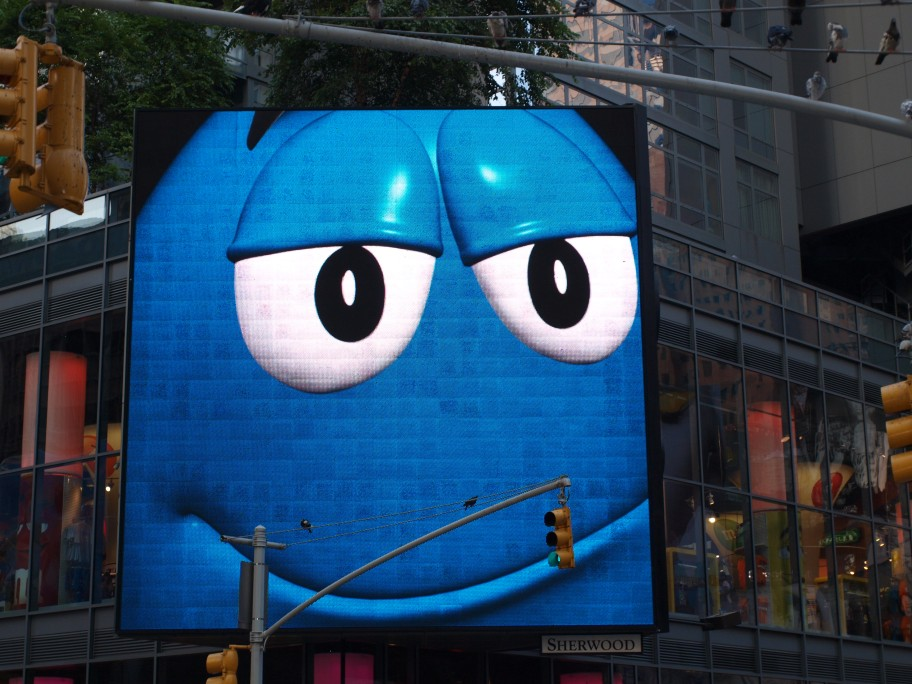
\includegraphics[width=0.398\linewidth]{figures/task2/mm.jpg}
	
\includegraphics[width=0.15\linewidth]{figures/task2/simple.PNG}
	\caption{The 3 test images. From left to right: future, mm and simple.}
	\label{fig:testimages}
\end{figure}

\subsubsection{Influence of using coordinates}

Figures \ref{fig:future:coords}, \ref{fig:mm:coords} and \ref{fig:simple:coords} illustrate the result of the segmentation by coloring each pixel by the color value of its associated centroid. We show the influence of the usage of coordinates for K=3 and K=5 clusters for each test image.
\begin{figure}[h!]
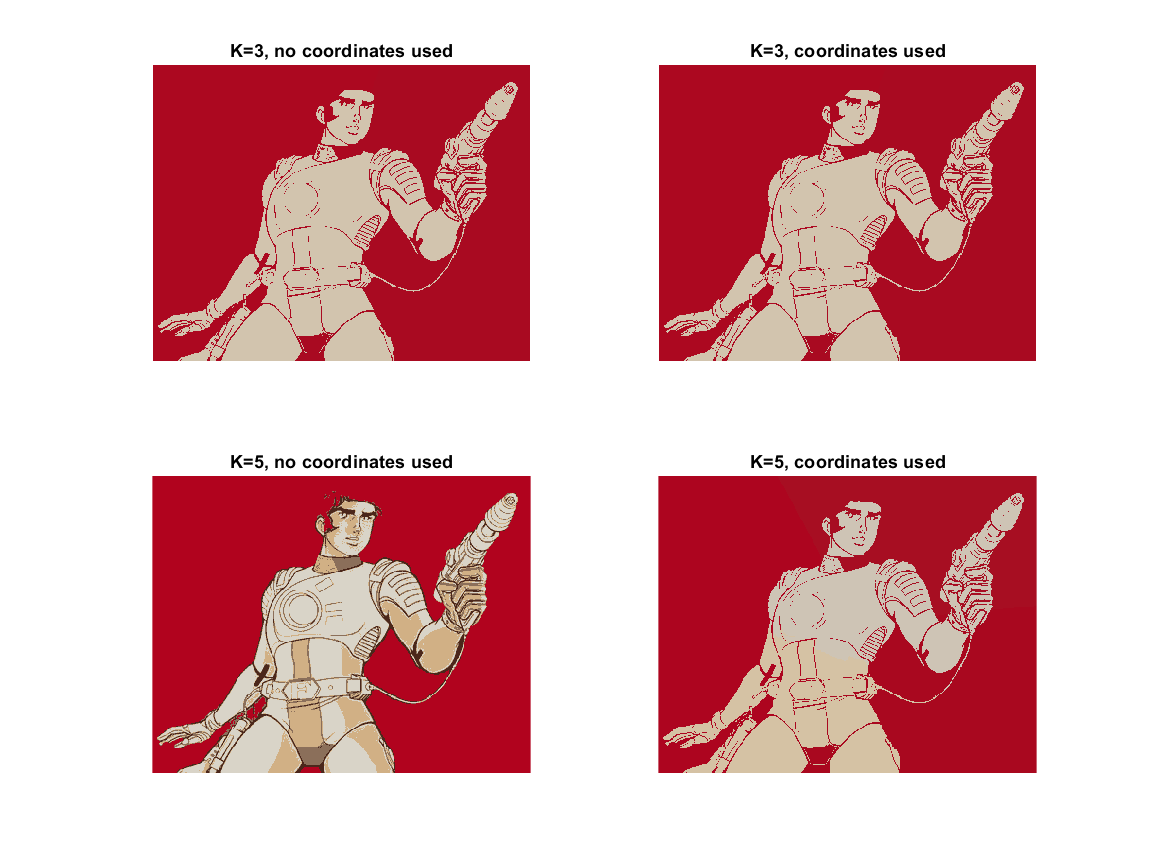
\includegraphics[width = 0.9\linewidth]{figures/task2/future_coordinates.png}
\caption{Coordinate experiment for \texttt{future.jpg}}
\label{fig:future:coords}
\end{figure}

For the "future.jpg" image we can see that the segmentation without using coordinates produces a pleasing result. It can separate the different colors very accurately. This is the case as the image contains only a limited number of colors, and all colors in a coherent region have the same color. For the clustering with coordinates it appears that the algorithm found less clusters than K. This is the case as the background gets segmented into multiple regions. This happens, because the pixels on the right and on the left have on one hand the same color, but are spatially far apart, so it makes sense to split the background in a left region and right region. For $K=5$ the image gets split into 3 background region a top part of person region and a bottom part of person region. We can see that not only the color is important, but also the spacial relation. We can already see here, that using the colors of the cluster center makes the inspection of the result hard, as several cluster, in particular for the case which uses coordinates, can have the same or very similar colors.
\begin{figure}
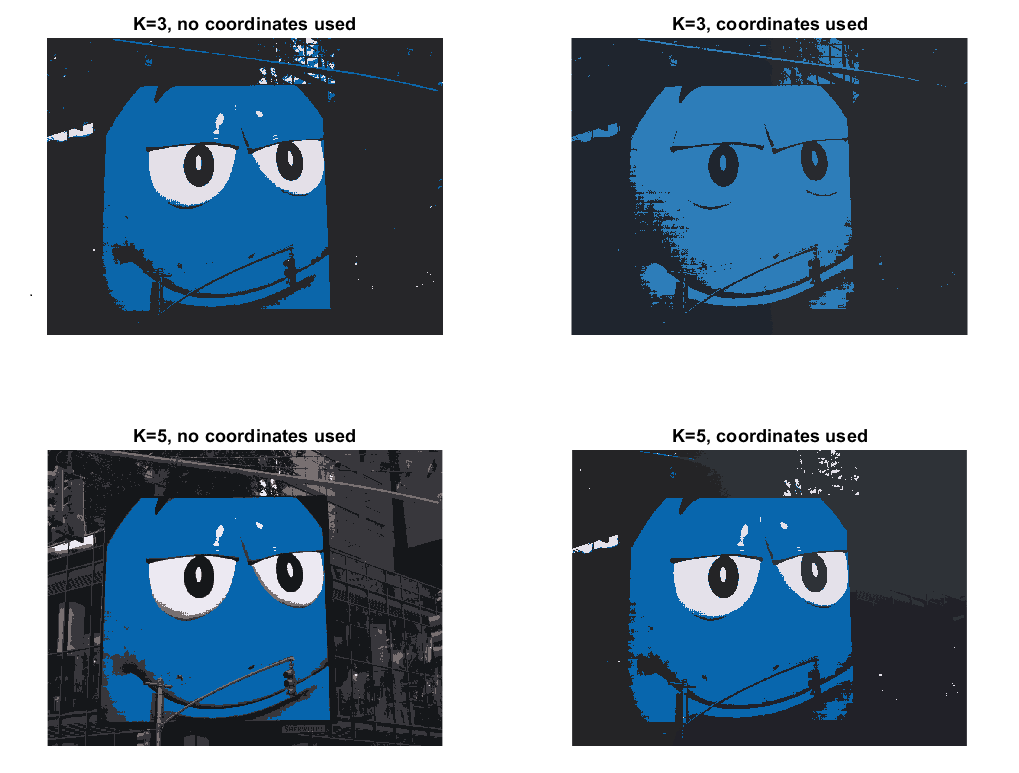
\includegraphics[width = 0.9\linewidth]{figures/task2/mm_coordinates.png}
\caption{Coordinate experiment for \texttt{mm.jpg}}
\label{fig:mm:coords}
\end{figure}


\begin{figure}[h]
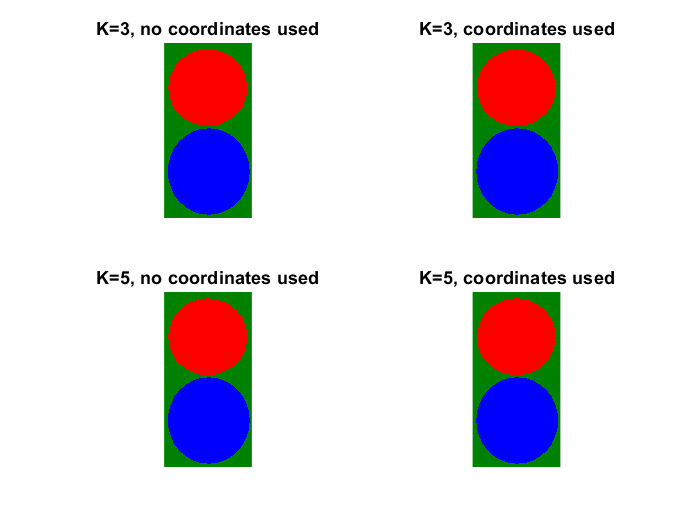
\includegraphics[width = 0.9\linewidth]{figures/task2/simple_coordinates.png}
\caption{Coordinate experiment for \texttt{simple.PNG}}
\label{fig:simple:coords}
\end{figure}


\FloatBarrier % keep figures above!

\section{Assignment 3: Scale-Invariant Blob Detection}
\label{sec:assignment3}

This assignment is about locating blobs of different sizes in images. A Laplacian blob detector is implemented and used in a scale-invariant way by convolving it with repeatedly blurred versions of the image to be analysed.
Interest point detectors in general are discussed in \cite{Szeliski}, and LoG as a feasible scale invariant detector in \cite{Lindeberg} and \cite{Mikolajczyk}.

\subsection{Problem definition}

Given an image, the problem is to find blob-like features of varying scale. In specific, the goals are to:
\begin{itemize}[noitemsep]
\item Implement a Laplacian of Gaussian (LoG) blob detector
\item Apply it to a reference image (\texttt{butterfly.jpg}) and an image of choice, and to also apply it to half-sized versions of the images
\item Indicate the found blobs by overlaying circles, with the circle radii being representative of the found blob's size
\item Plot the LoG response over all scales at a specific key point for both the original and half-sized image
\item Discuss the results
\end{itemize}

\subsection{Methodology}
\label{sec:a3:methodology}

The detector parameters and image filename (\texttt{sigma0, k, level, thresh, FILENAME}) are defined in the first couple of lines of the implementation and can easily be changed there to experiment with different values.
After loading the image, we create a scale space matrix of depth \texttt{level}, each level corresponding to a specific value of $\sigma$.
The original image is convoluted with an LoG-filter of size proportional to increasing values of $\sigma$ ($= \sigma_0 k^{level-1}$), and the result is stored in the scale-space-matrix, so that each level represents the filter response to an increasingly blurred version of the image.
In order to detect blobs independently of the intensity relative to their background, we store the absolute value of the filter response.

Non-maxima-suppression is then performed on the scale-space-matrix, leaving only those elements non-zero, which are larger than all of their 26 immediate neighbours in the three-dimensional matrix. Each of these remaining points corresponds to the centre of a detected blob (dimension 1 and 2 of the matrix), and the blob's size (dimension 3: $\sigma$).

\subsection{Experiments}

We experimented with two images (\texttt{butterfly.jpg} and \texttt{dalmation.png}) and used the blob detector on both the original as well as a half-sized version of each. Figure \ref{fig:a3:general} demonstrates the results for a specific set of parameters ($\sigma_0=2, k=1.25, threshold=0.20, levels=10$). It can be seen, that the detector finds most blobs in a scale-invariant way; specifically matching blobs are found in both scalings of an image, if both their original radius and half sized radius are in the range covered by parameters $\sigma, k, levels$: the size of detected blobs is limited by the range of $\sigma$-values; only blobs whose radius lies in $r_{min} \leq r \leq r_{max}$ ($r_{min} = \sigma_0 \sqrt{2}$ and $r_{max} = \sigma_0 k^{levels-1}  \sqrt{2}$) will be found. Scale invariance can break in one of three ways: Either a blob is too large to be found in the original image, but small enough so that its half-sized appearance in the half-sized image is detected (e.g. the large blob at the right wing tip of the butterfly in Figure \ref{fig:a3:general}, bottom right image); or it is too small to be found in the half-sized image, but large enough to be detected in the original (e.g., the small blobs on the hind paw of the Dalmatian in Figure \ref{fig:a3:general}, top left image). A third possible way, which we did not observe, could arise if the downscaling process of the image alters the intensity values in such a way, that a potential blob is excluded from one image during non-maxima-suppression (due to thresholding), but not in the other.

\begin{figure}[h]
	\centering
	\begin{tabular}{cc}
		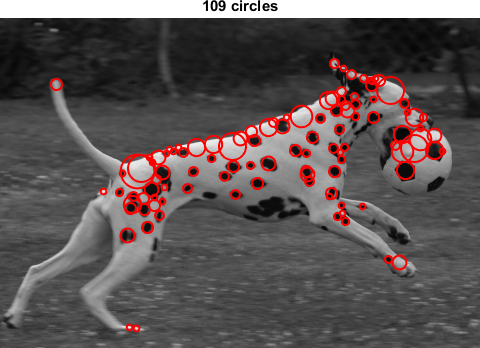
\includegraphics[width=0.5\textwidth]{figures/a3_dalmation_k020_full.png} &
		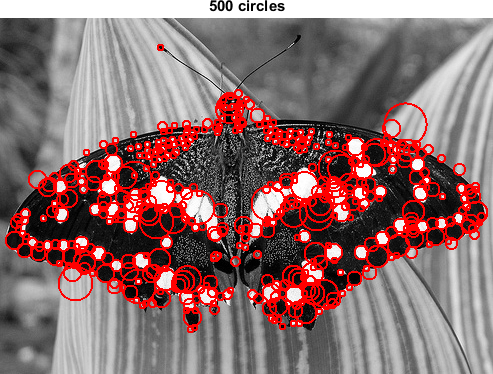
\includegraphics[width=0.5\textwidth]{figures/a3_butterfly_k020.png} \\
		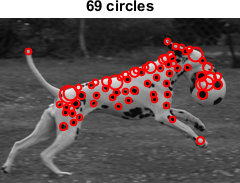
\includegraphics[width=0.25\textwidth]{figures/a3_dalmation_k020_half.png} &
		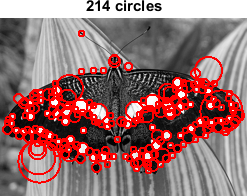
\includegraphics[width=0.25\textwidth]{figures/a3_butterfly_k020_small.png} \\
	\end{tabular}
	\caption{LoG blob detector applied to two different images and to half-sized versions of them. Parameters: $\sigma_0=2, k=1.25, threshold=0.20, levels=10$.}
	\label{fig:a3:general}
\end{figure}

We experimented with different threshold values to find satisfactory values; see Figure \ref{fig:a3:thresholds} for results. Obviously, the lower the threshold is, the more blobs are found. Our final choice of $threshold=0.20$ was obtained by a subjective judgement, i.e. if we considered the results to be ``real'' blobs or not. This leads to ambiguities though; for example, we would consider the blotches in the bottom left background (Figure \ref{fig:a3:thresholds}, top left image) to be more ``real'' blobs than the leaf segment above the right wing; however with increasing threshold the blotches disappear first, while the leaf segments persist.

\begin{figure}[h]
	\centering
	\begin{tabular}{cc}
	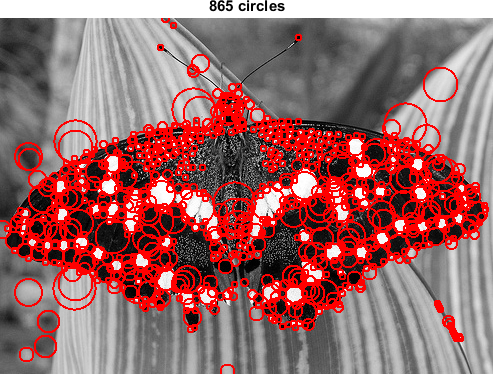
\includegraphics[width=0.5\textwidth]{figures/a3_butterfly_k015.png} &
	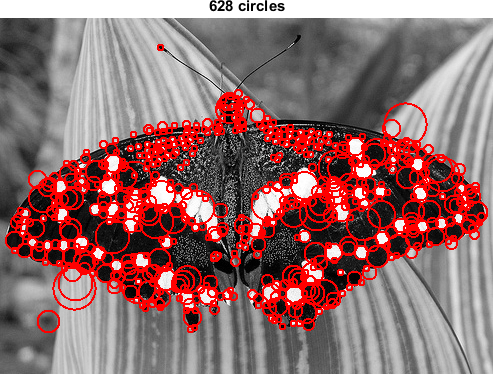
\includegraphics[width=0.5\textwidth]{figures/a3_butterfly_k018.png} \\
	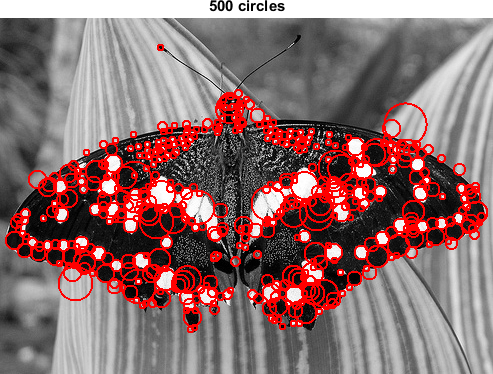
\includegraphics[width=0.5\textwidth]{figures/a3_butterfly_k020.png} &
	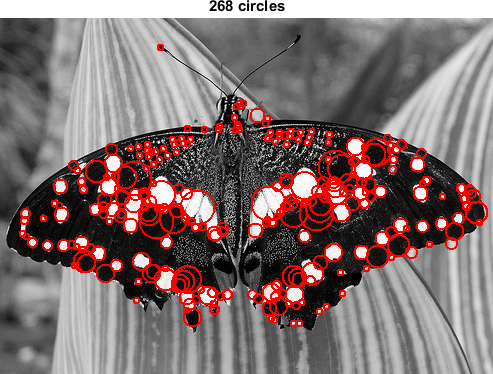
\includegraphics[width=0.5\textwidth]{figures/a3_butterfly_k025.png} \\
	\end{tabular}
	\caption{Illustration of the effect of different thresholds $t$. Top left: $t=0.15$. Top right: $t=0.18$. Bottom left: $t=0.20$. Bottom right: $t=0.25$.}
	\label{fig:a3:thresholds}
\end{figure}

Additionally, we examined the LoG response over all scale levels for specific key points (blob centres). Figure \ref{fig:a3:logresponse} shows the response for two distinct key points of the butterfly image. When comparing the responses of the original image to those of the half-sized version, it can be seen that the extremal values appear on different scale levels. E.g., for the key point on the left side of Figure \ref{fig:a3:logresponse}, we find the extrema (minima in this case) at level 9 ($\sigma_{full}=11.92$) for the full resolution and level 6 ($\sigma_{half}=6.10$) for the half-sized blob respectively. Indeed $\sigma_{full} : \sigma_{half} \approx 2:1$ as expected, i.e. the radius in the full image is twice as large.

It can also be seen that the initial LoG response is sensitive to the gradient direction. E.g., a bright blob on dark background produces a minimal response at the correct scale, while a dark blob on bright background produces a maximal response. Since we do not care about the gradient direction to detect blobs, we only search for maxima of the \textit{absolute} response, as described in Section \ref{sec:a3:methodology}.

\begin{figure}[h]
	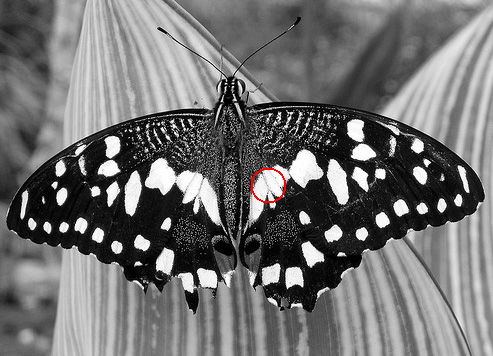
\includegraphics[width=0.5\textwidth]{figures/a3_butterfly_keypoint.png}
	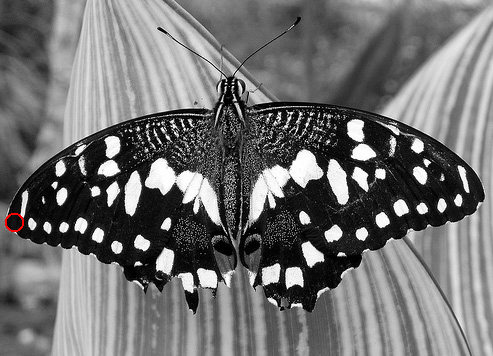
\includegraphics[width=0.5\textwidth]{figures/a3_butterfly_keypoint_2.png}
	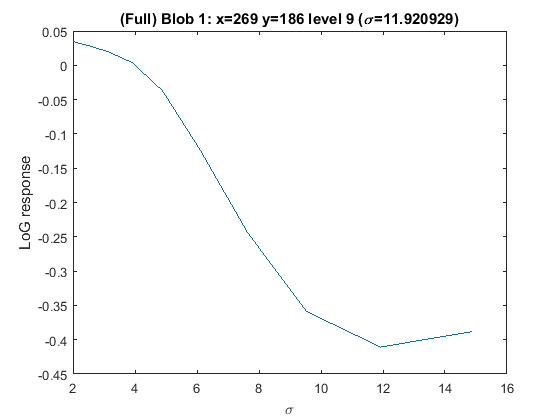
\includegraphics[width=0.5\textwidth]{figures/a3_butterfly_log_full.png}
	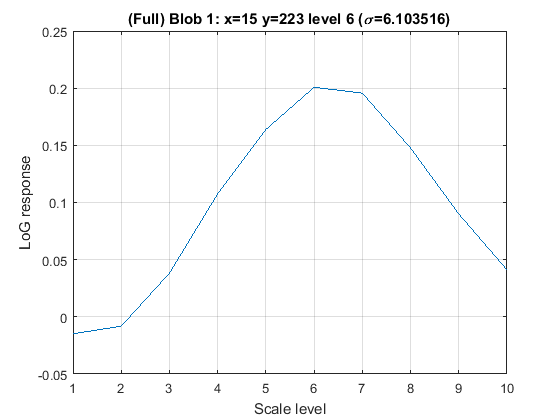
\includegraphics[width=0.5\textwidth]{figures/a3_butterfly_log_full_2.png}
	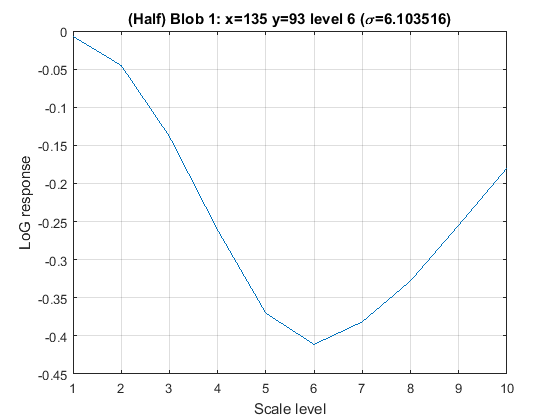
\includegraphics[width=0.5\textwidth]{figures/a3_butterfly_log_half.png}
	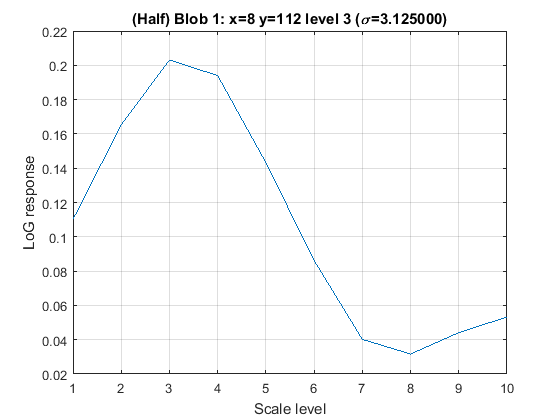
\includegraphics[width=0.5\textwidth]{figures/a3_butterfly_log_half_2.png}
	\caption{LoG response for two selected key points. The top row shows the chosen key point, the second and third rows show the LoG response for the full-sized and half-sized image. Left: A white-on-black blob (negative LoG response), right: a black-on-white blob (positive LoG response).}
	\label{fig:a3:logresponse}
\end{figure}


\FloatBarrier % keep figures above!


%% *********
%% Bibliography
%% *********

\fontsize{9}{10pt}
\bibliographystyle{plain}

\begin{thebibliography}{10}

% uncomment/add used references

\bibitem{Lindeberg}
Lindeberg,~T.,
\newblock ``Scale-space theory: A basic tool for analysing structures at different scales'',
\newblock \textit{Journal of Applied Statistics}, 21(2):224–270, 1994.

\bibitem{Mikolajczyk}
Mikolajczyk,~K.,
\newblock ``Detection of local features invariant to affine transformations'',
\newblock \textit{PhD thesis, INPG, Grenoble}, 2002.

\bibitem{Szeliski}
Szeliski,~R.,
\newblock \textit{Computer Vision: Algorithms and Applications},
\newblock Springer, 2010.
\newblock \url{http://szeliski.org/Book/drafts/SzeliskiBook_20100903_draft.pdf}.

\end{thebibliography}

\end{document}

%%% Local Variables: 
%%% mode: latex
%%% TeX-master: t
%%% End: 

